% Compile twice with XeLaTeX from the report directory.
\documentclass[UTF8,a4paper,zihao=-4,fontset=windows]{ctexart}
\usepackage[margin=22mm,headheight=15pt]{geometry}
\usepackage{graphicx,booktabs,tabularx,amsmath,xcolor,fancyhdr}
\usepackage[unicode,hidelinks]{hyperref}
\definecolor{accent}{HTML}{235D80}
\ctexset{section={format=\Large\bfseries\color{accent}},subsection={format=\normalsize\bfseries}}
\pagestyle{fancy}
\fancyhf{}
\fancyhead[L]{\small Imagenette 图像分类实验}
\fancyhead[R]{\small 第二次学习规划}
\fancyfoot[C]{\small\thepage}
\setlength{\parskip}{4pt}
\linespread{1.08}
\renewcommand{\arraystretch}{1.22}
\makeatletter
\newcommand{\captionof}[2]{\begingroup\def\@captype{#1}\caption{#2}\endgroup}
\makeatother
\graphicspath{{../outputs/}}
\hypersetup{pdftitle={Imagenette图像分类实验报告},pdfsubject={MLP、CNN与水平翻转对照}}
\begin{document}
\begin{center}
{\LARGE\bfseries Imagenette 图像分类实验报告}\par
\vspace{5pt}
{\large MLP、CNN 与随机水平翻转对照}\par
{\small 基于已保存的训练历史、配置及最终测试结果}
\end{center}

\section{任务、数据与运行环境}
本实验比较 MLP、CNN 与 CNN-Flip 三种方案，理解图片如何经过前向传播、损失计算、反向传播和优化器更新形成分类能力，并观察卷积结构及训练数据增强的作用。三组均从随机初始化开始，训练 20 轮，不使用预训练权重。

Imagenette-160 包含 tench、English springer、cassette player、chain saw、church、French horn、garbage truck、gas pump、golf ball 和 parachute 共 10 类。使用原始类别文件夹标签，不使用噪声标签 CSV。

\begin{center}
\begin{tabular}{lll}
\toprule
数据集合 & 来源 & 图片数\\\midrule
训练集 & 官方 train 分层划分 & 7,575\\
内部验证集 & 官方 train 分层划分 & 1,894\\
最终测试集 & 官方 val 全部图片 & 3,925\\\bottomrule
\end{tabular}
\end{center}
划分 seed 为 42；三组共用固定清单和类别映射。验证集负责选择 epoch，测试集保留到选模结束后评价，不能根据测试结果反复调参。

运行环境为 Windows 11、Python 3.13.7（项目 \texttt{.venv}）、PyTorch 2.7.1+cu118、TorchVision 0.22.1+cu118，GPU 为 NVIDIA GeForce RTX 3070 Ti Laptop GPU。

\section{输入处理与模型结构}
统一将图片转换为 RGB，短边缩放至 160、中心裁剪为 $160\times160$，再将像素除以 255。输入 batch 形状为 $B\times3\times160\times160$。只有 CNN-Flip 的训练图片在裁剪后、转张量前，以 0.5 概率水平翻转；验证和测试不翻转。除以 255 是固定比例缩放，不需要估计数据均值和方差。

\textbf{MLP：}展平为 76,800 维，经 256 维全连接层、ReLU，再输出 10 个类别得分。总参数量为 19,663,626。展平保留像素与固定位置顺序，但全连接层没有卷积的局部连接与权重共享结构。

\textbf{CNN：}四组 $3\times3$ 卷积、ReLU 与 $2\times2$ 最大池化；通道依次为 32、64、128、128，卷积 stride=1、padding=1，池化 stride=2。空间尺寸从 160 依次降至 80、40、20、10；自适应平均池化至 $4\times4$，展平为 2,048 维，经 256 维全连接层、ReLU 和 10 维输出层。总参数量为 767,946。CNN-Flip 使用相同结构。

\clearpage
\section{训练协议与学习曲线}
共同设置为 seed=42、Adam、固定学习率 0.001、weight decay=0、batch size=64、交叉熵损失和 20 epoch。每批清除旧梯度，前向生成 logits，计算 loss，再由 backward 计算梯度、Adam 更新参数。模型末尾不额外加入 softmax。

CNN 和 CNN-Flip 的初始权重 SHA256 相同，各自独立训练。两组的预期干预是水平翻转；相同 seed 与初始权重不意味着增强及打乱的随机过程逐步相同。每组按最高内部验证 accuracy 保存权重，并列保留较早轮次，训练满 20 轮。

\begin{center}
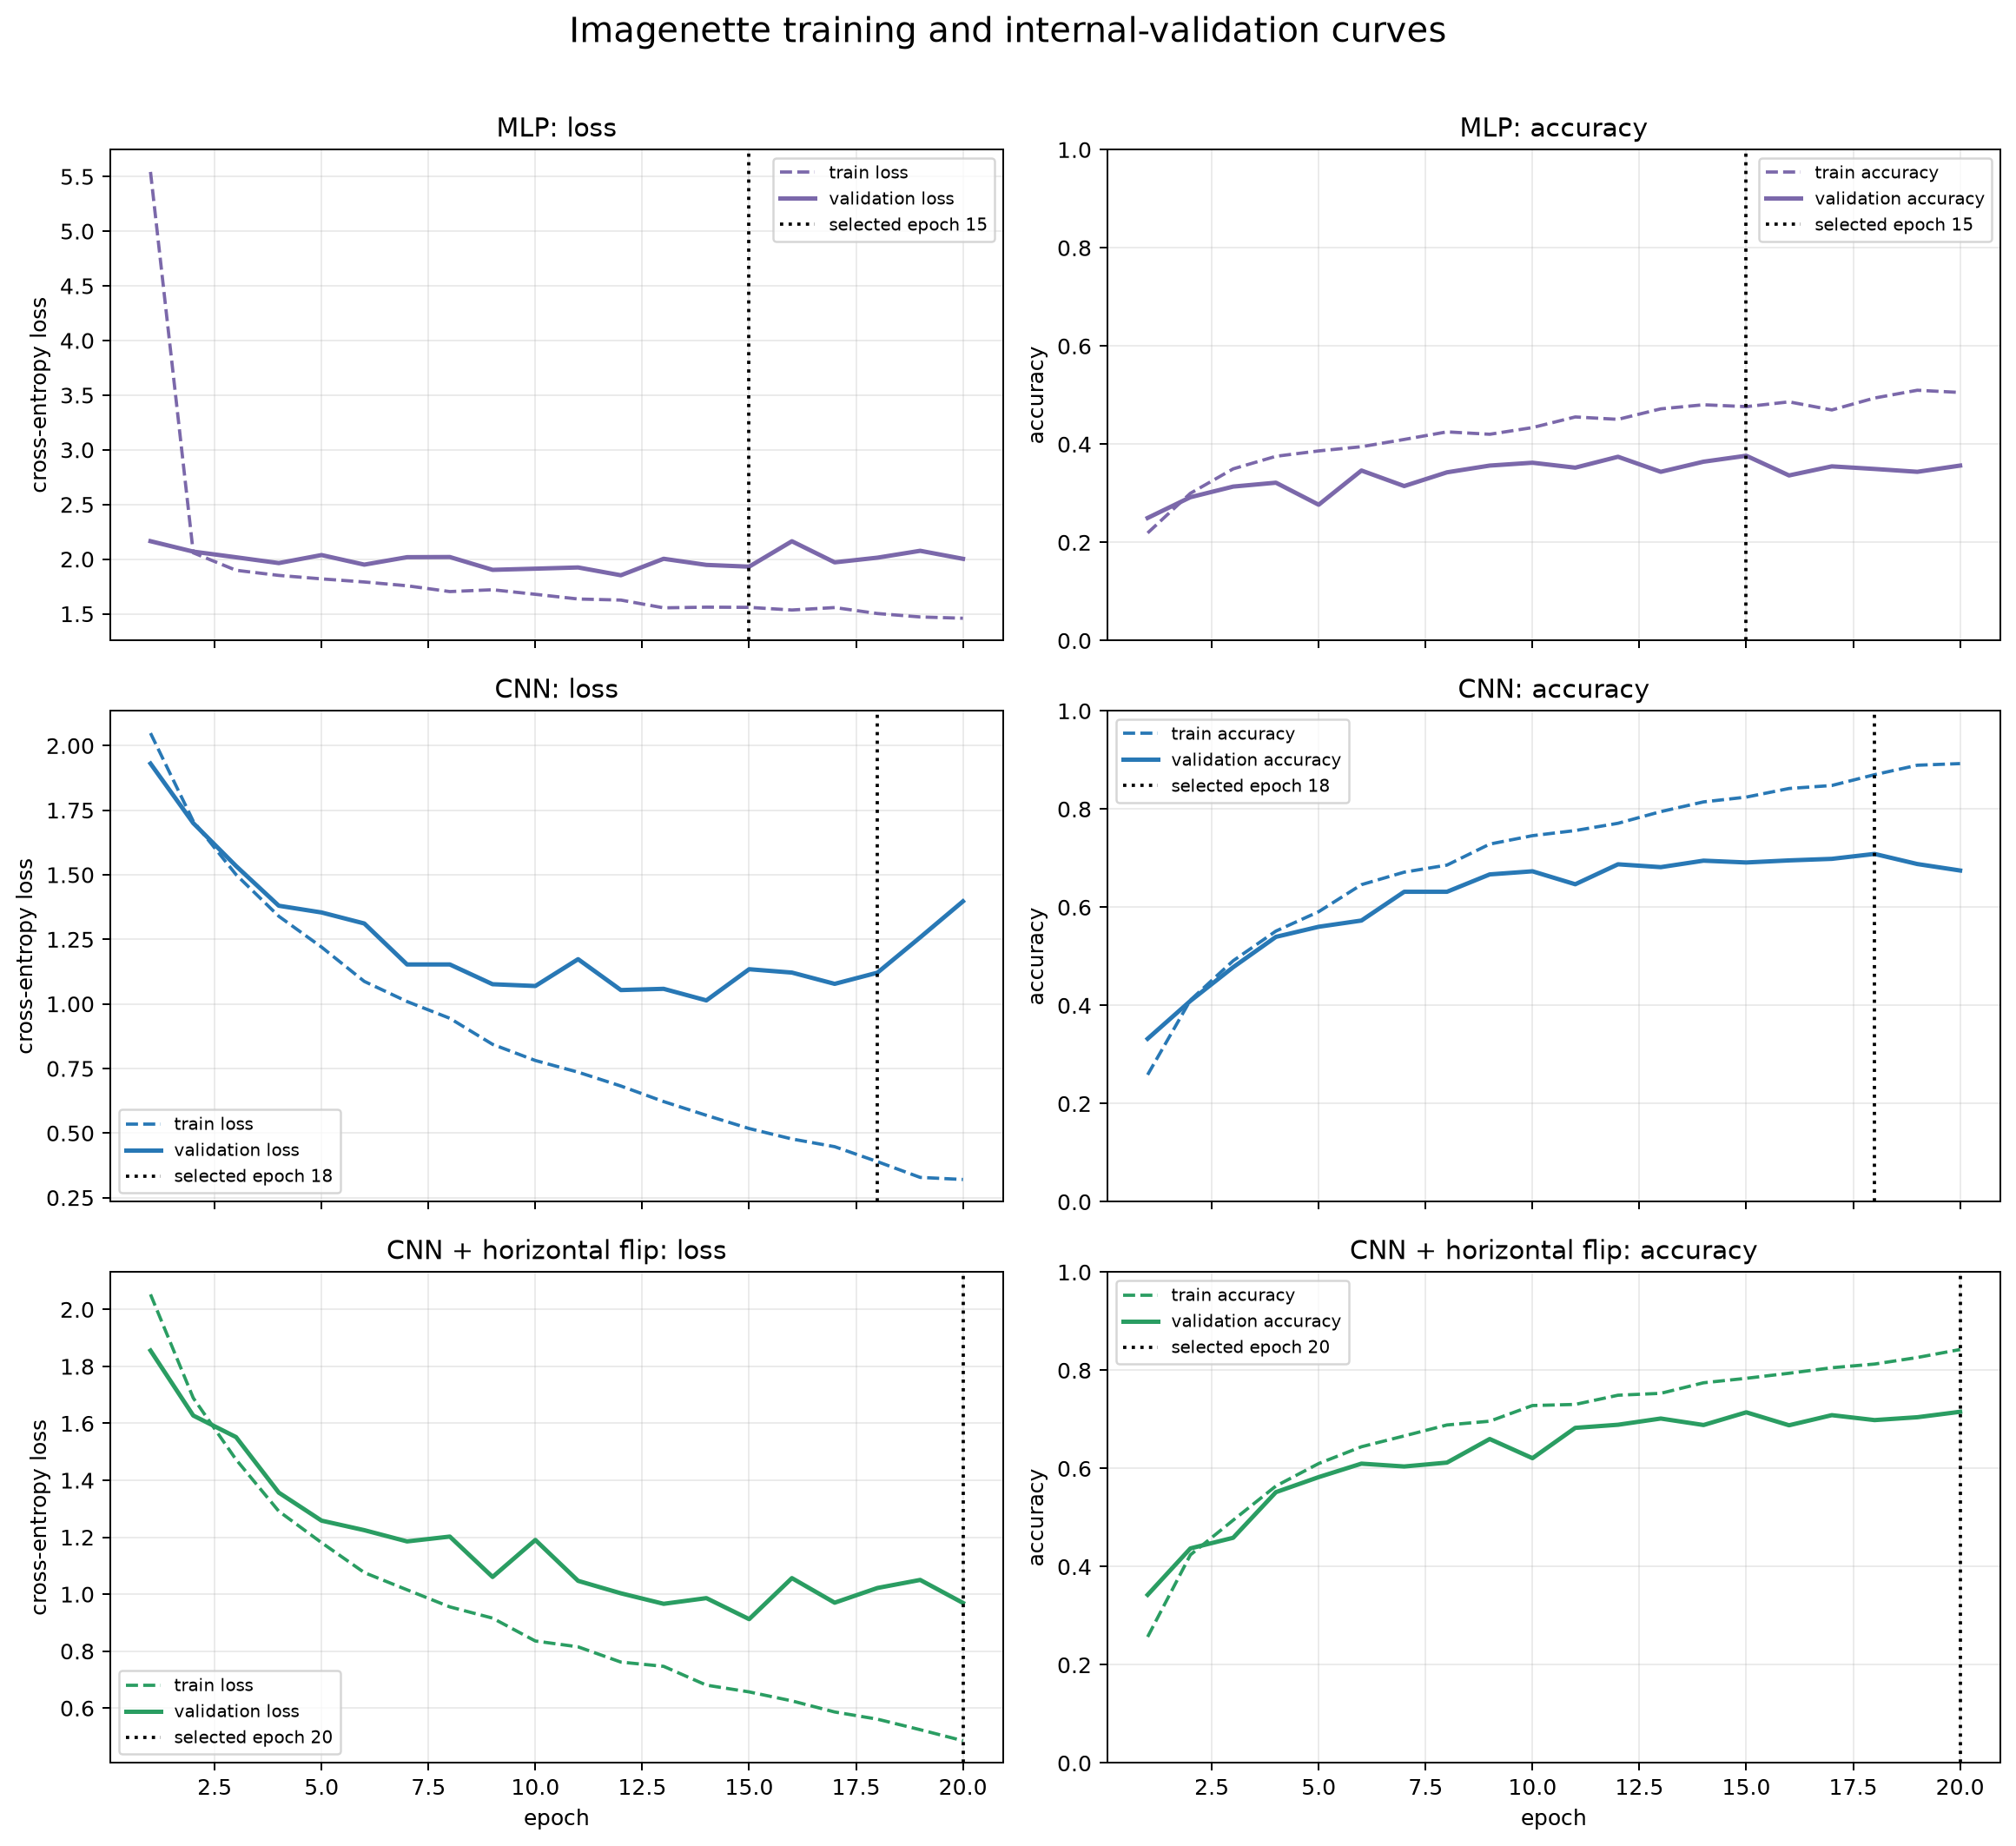
\includegraphics[width=\linewidth,height=0.59\textheight,keepaspectratio]{summary/training-curves.png}
\captionof{figure}{三组训练与内部验证曲线；黑色竖虚线标出按验证 accuracy 选中的轮次。}
\end{center}

MLP 在第 15 轮后验证 accuracy 未再提升；CNN 在第 18 轮后训练表现继续改善、验证表现回落，提示过拟合。CNN-Flip 在第 20 轮达到最佳验证 accuracy，训练 accuracy 较普通 CNN 低而验证表现略高。该现象与增强改善泛化相符，但训练指标来自逐 batch 更新过程且包含增强，不能将差距完全归因于“记忆程度”。

\clearpage
\section{最终测试与三组比较}
在新进程中重载各自最佳权重，以 \texttt{eval()} 和 \texttt{no\_grad()} 对相同的 3,925 张测试图片预测。预测类别取 10 个 logits 的最大值位置。后续为了更新样例图再次运行同一权重评估，是产物复核，不是新的独立实验。

\begin{center}
\small
\begin{tabular}{lrrrrr}
\toprule
模型 & 参数总量 & 选中轮次 & 验证 Acc. & 测试 Acc. & Macro-F1\\\midrule
MLP & 19,663,626 & 15 & 0.3765 & 0.3651 & 0.3558\\
CNN & 767,946 & 18 & 0.7086 & 0.7108 & 0.7110\\
CNN-Flip & 767,946 & 20 & 0.7154 & \textbf{0.7266} & \textbf{0.7265}\\\bottomrule
\end{tabular}
\captionof{table}{结果来自每组 metrics.json 与 run\_metadata.json；数值四舍五入至四位小数。}
\end{center}

\begin{center}
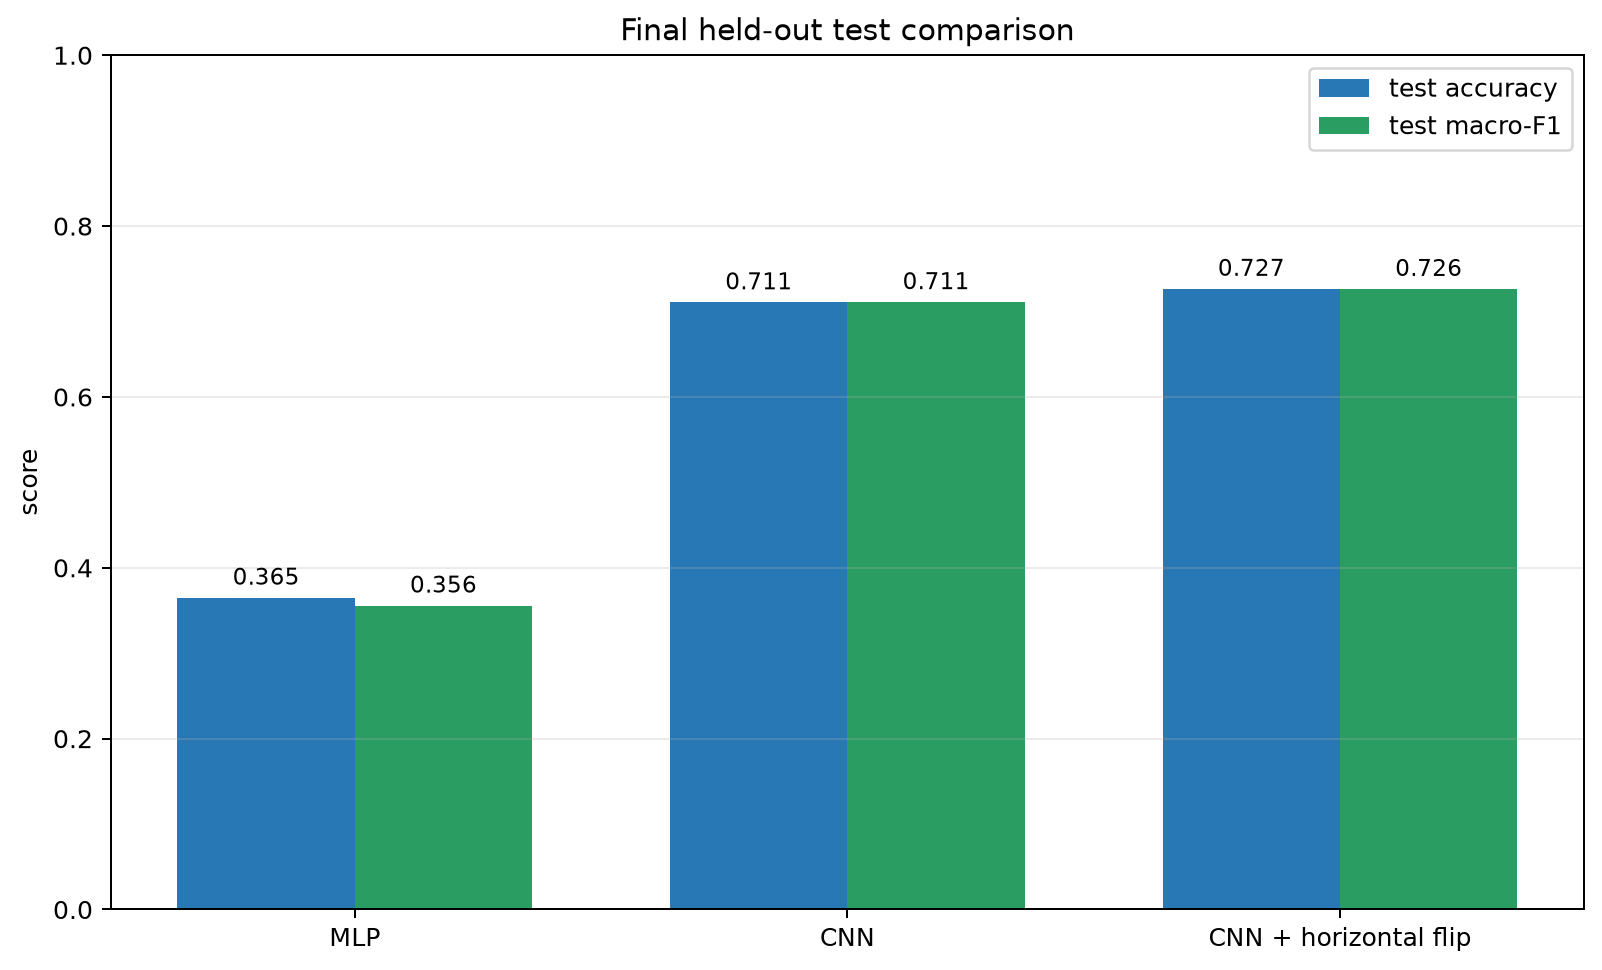
\includegraphics[width=0.94\linewidth]{summary/test-comparison.png}
\captionof{figure}{最终测试 Accuracy 与 Macro-F1 对比。}
\end{center}

CNN 比 MLP 的测试 accuracy 高约 34.57 个百分点，同时参数更少，说明本配置下利用局部空间结构比单纯增加全连接参数更有效。两者参数量和计算量不同，本比较不是等参数量实验。

CNN-Flip 比 CNN 的测试 accuracy 高约 1.58 个百分点，macro-F1 高约 1.55 个百分点。只有固定 seed=42 的一次实验，不能据此判断统计显著性或声称所有任务均会受益。

Accuracy 统计全部图片中预测正确的比例；Macro-F1 对每类 F1 等权平均，F1 综合该类精确率和召回率。两者接近不能证明所有类别表现均衡，应结合逐类召回率和混淆矩阵。

\clearpage
\section{混淆矩阵与逐类表现}
\begin{center}
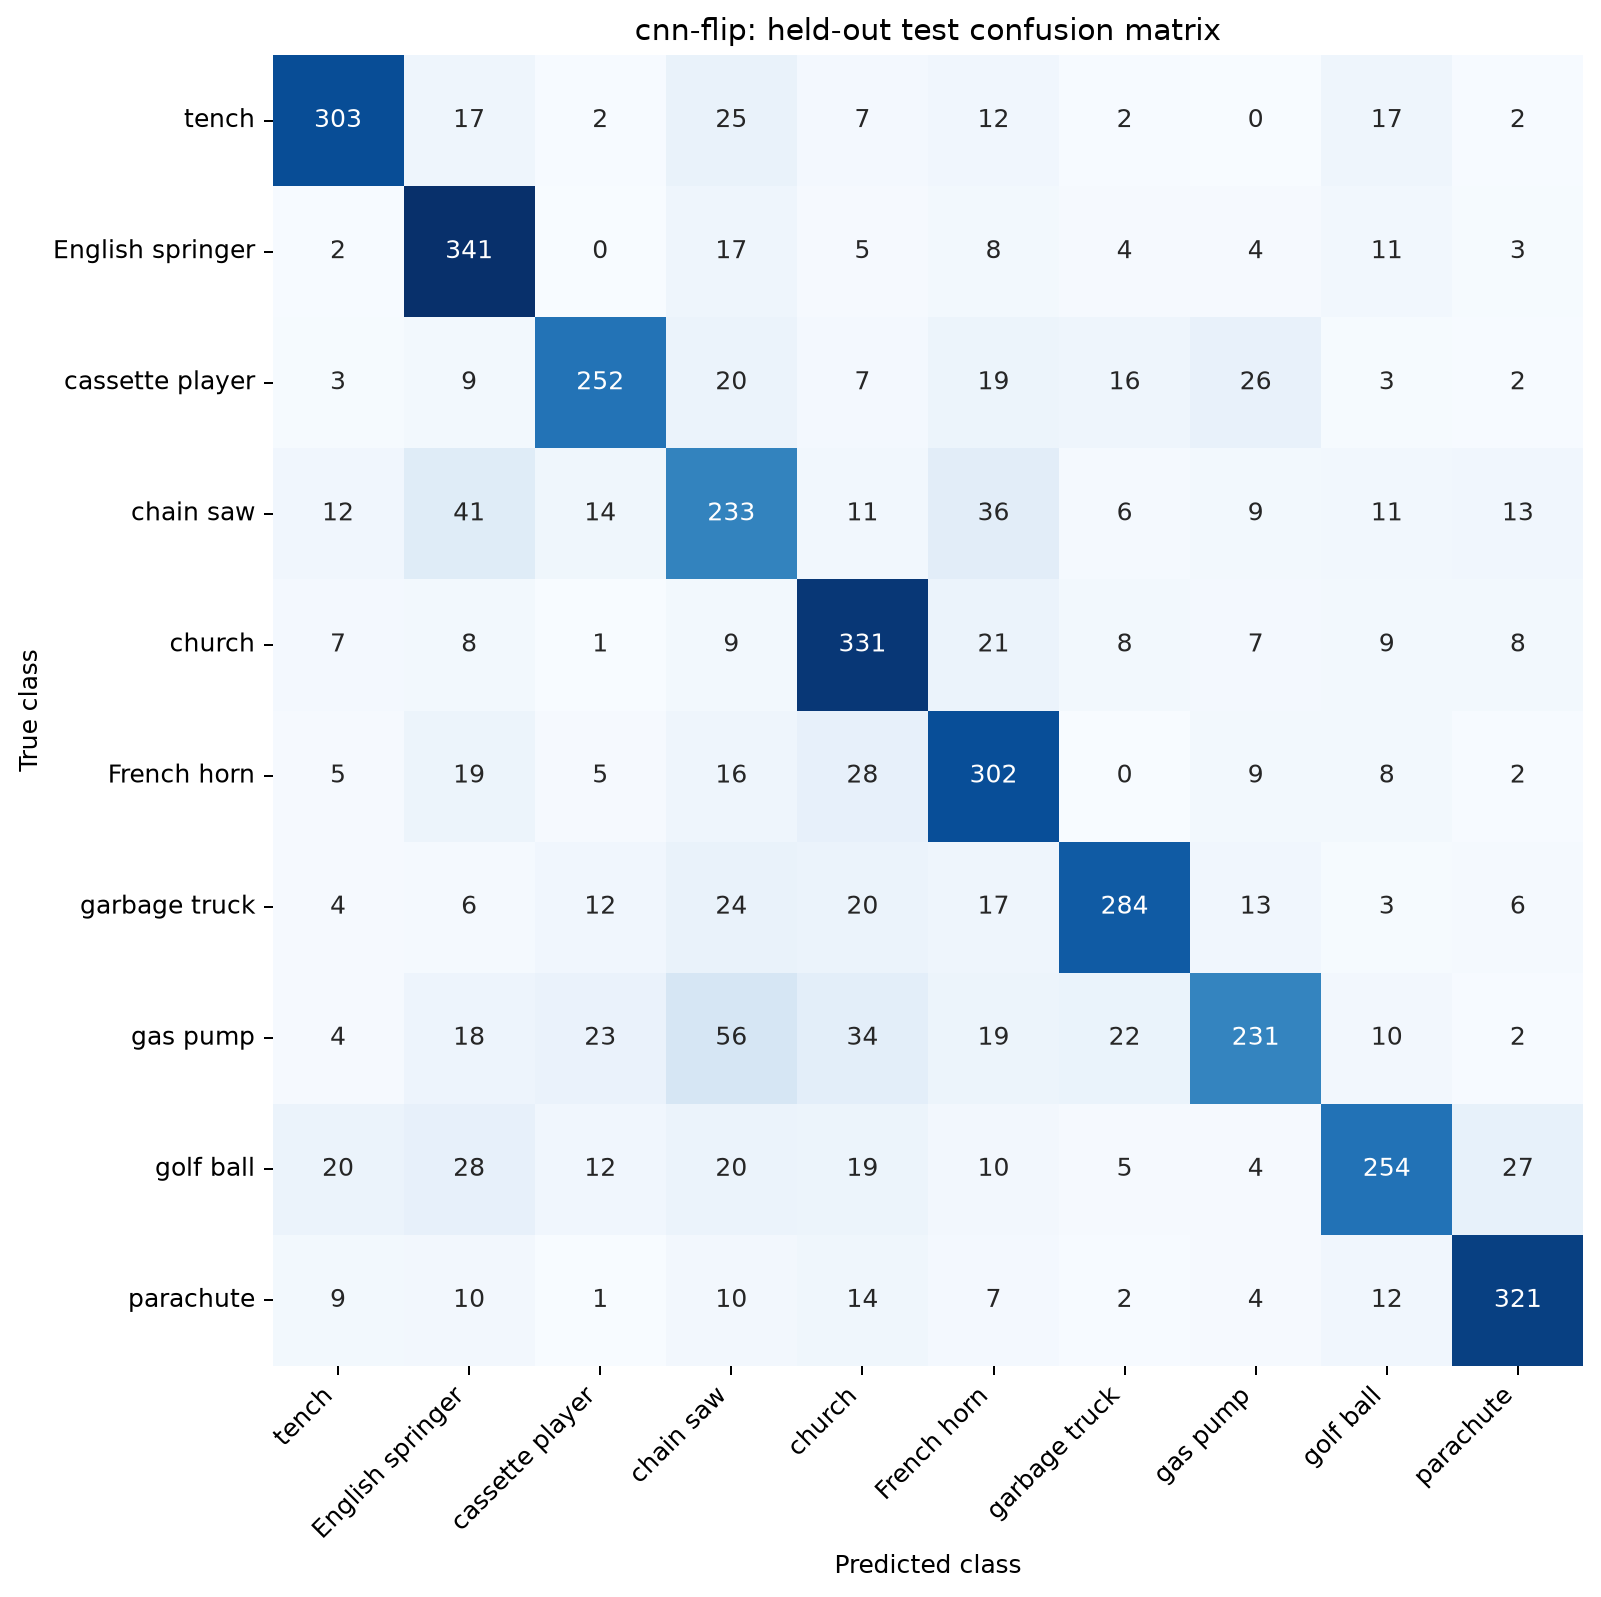
\includegraphics[width=0.86\linewidth]{cnn-flip/confusion-matrix.png}
\captionof{figure}{CNN-Flip 的测试混淆矩阵；行为真实类别，列为预测类别，显示原始数量。}
\end{center}

例如 English springer 正确识别 $341/395$，召回率约 86.33\%；gas pump 正确识别 $231/419$，召回率约 55.13\%，其中 56 张错分为 chain saw。跨类别比较不能只看对角线颜色或数量，应看相对于该类总数的比例。

\begin{center}
\begin{tabular}{lrr}
\toprule
类别 & CNN 召回率 & CNN-Flip 召回率\\\midrule
English springer & 0.8051 & 0.8633\\
church & 0.7066 & 0.8093\\
chain saw & 0.5363 & 0.6036\\
gas pump & 0.7017 & 0.5513\\
garbage truck & 0.7943 & 0.7301\\\bottomrule
\end{tabular}
\captionof{table}{部分逐类召回率：整体改善不等于每一类都改善。完整十类结果保存在各组 metrics.json。}
\end{center}

\clearpage
\section{正确与错误样例分析}
\begin{center}
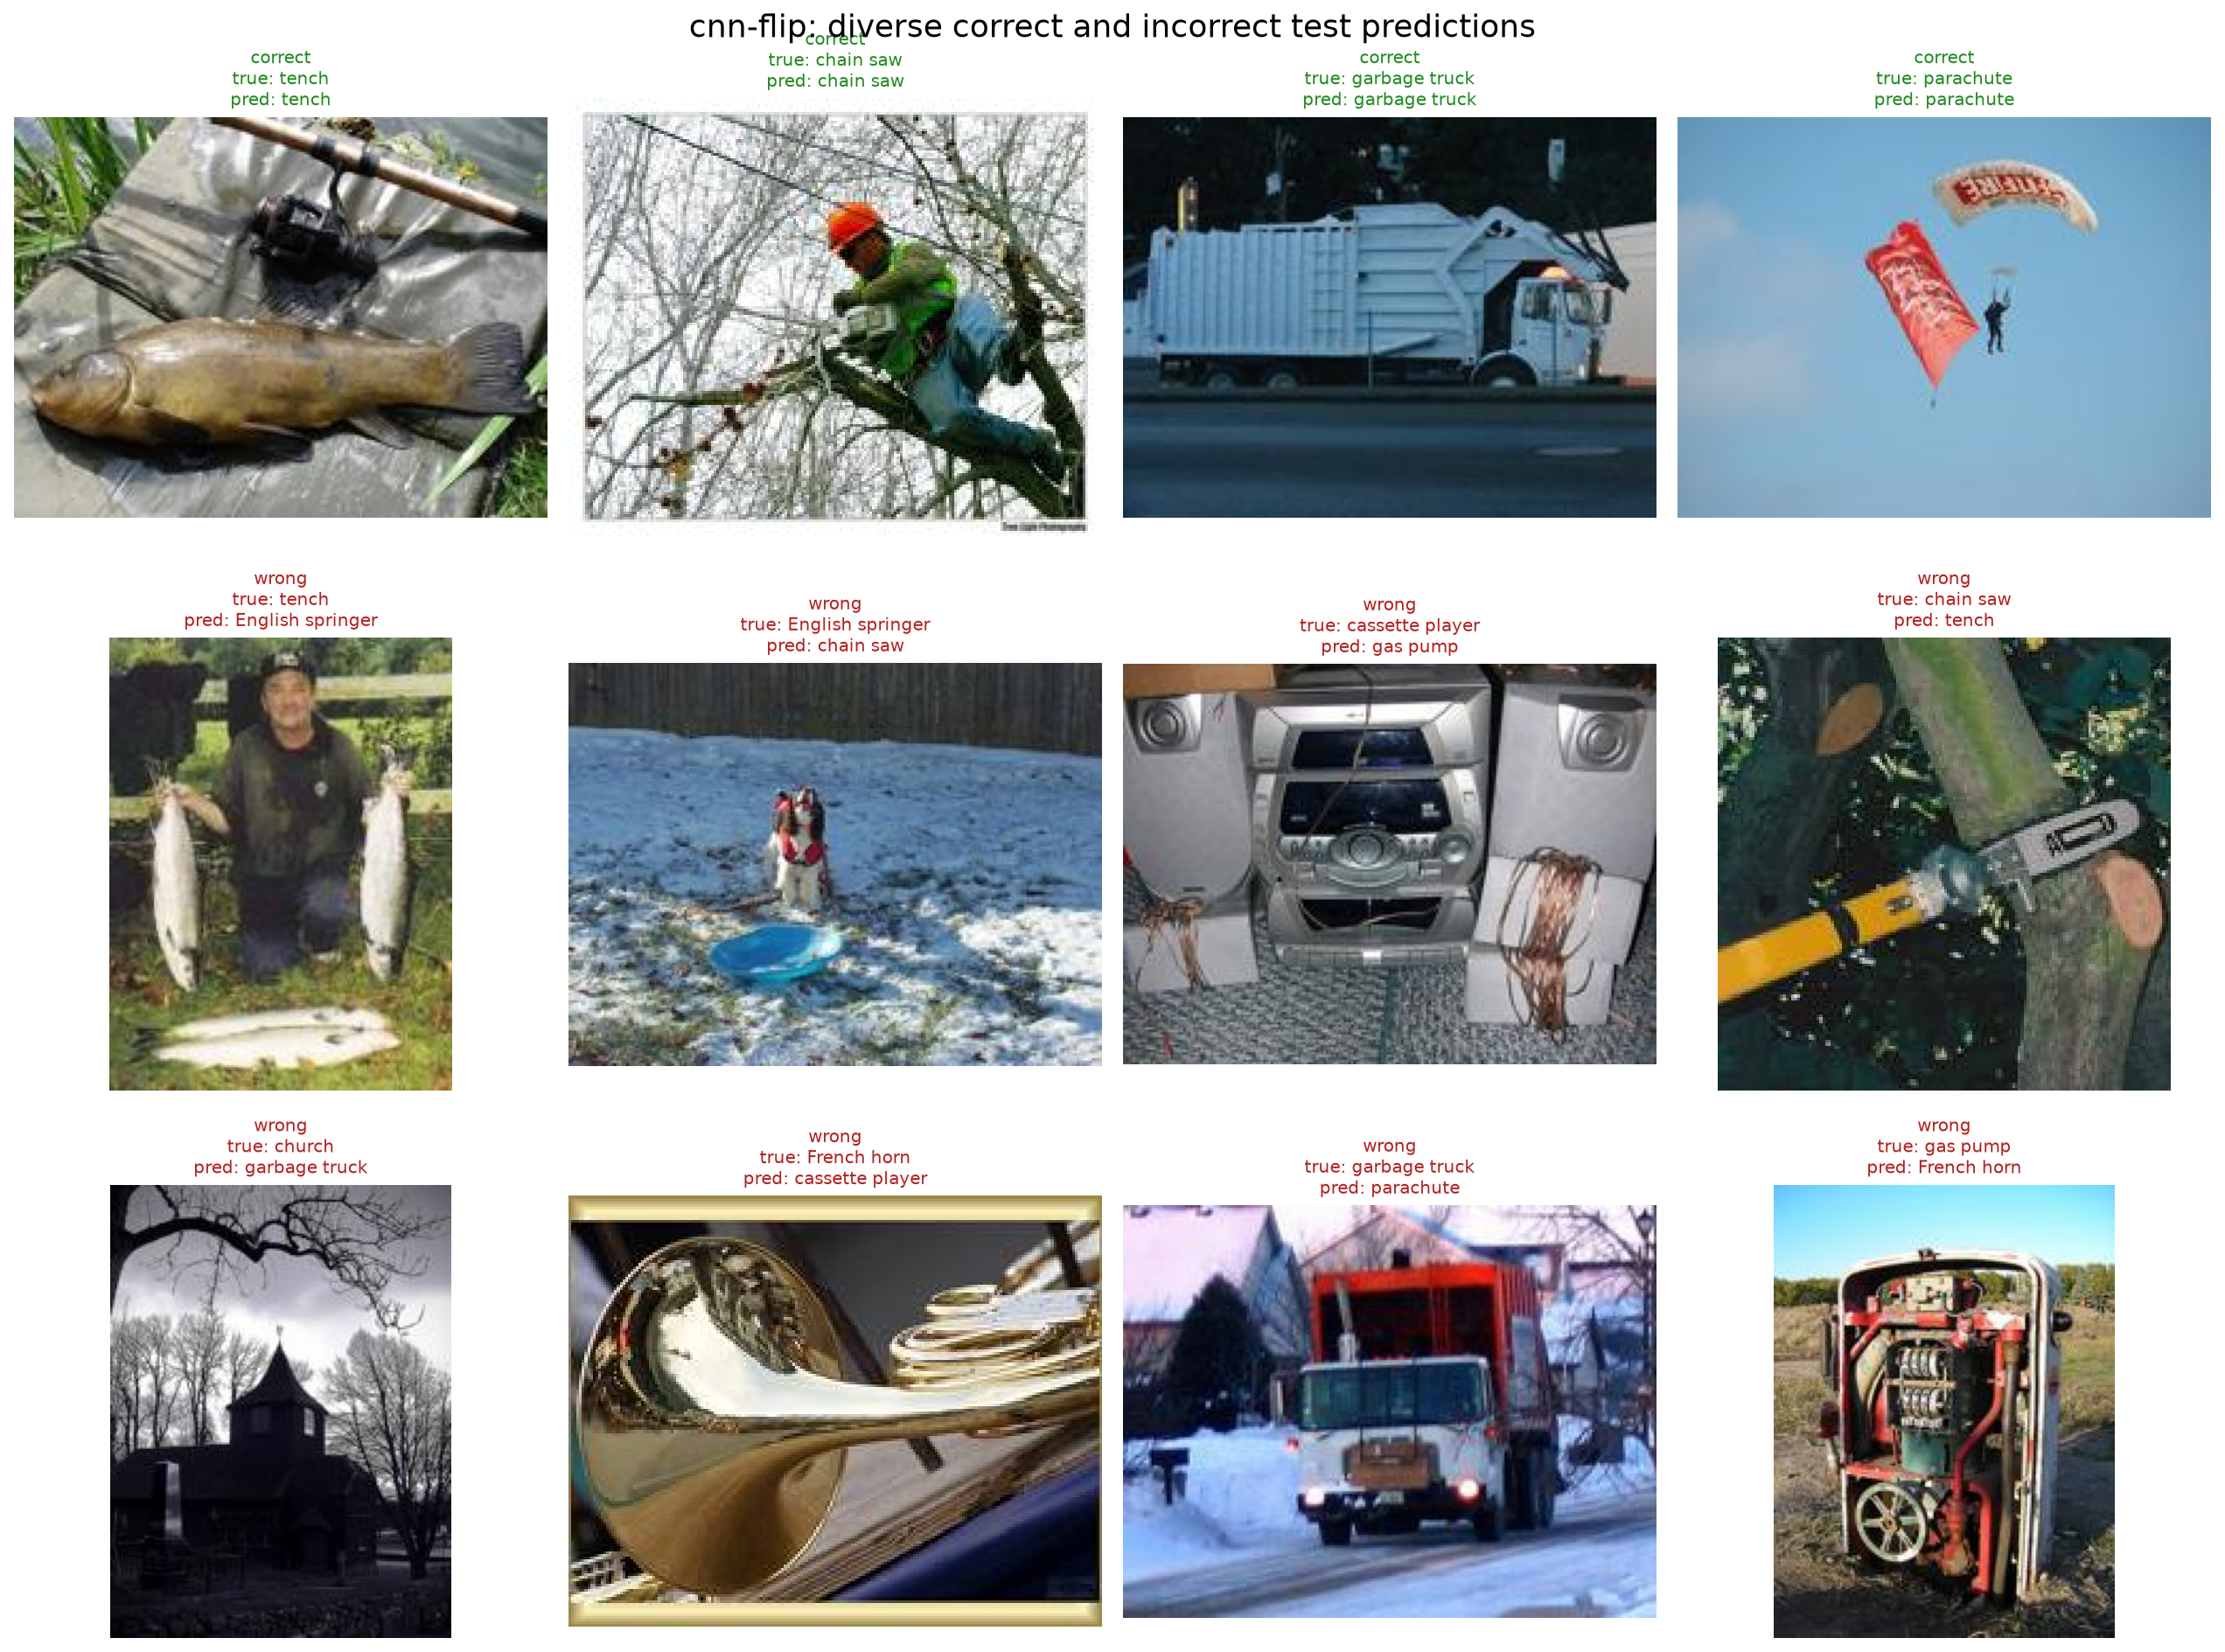
\includegraphics[width=\linewidth]{cnn-flip/examples.png}
\captionof{figure}{CNN-Flip 的 4 张正确与 8 张错误样例；标注真实和预测类别。}
\end{center}

图中的狗较小且处于雪地背景，教堂偏暗并被树枝包围，圆号展示局部金属结构，加油机露出内部机械部件。这些现象提示主体尺度、光照、背景与局部外观可能影响预测，但仅凭错误图片不能确定模型真实依赖了哪种线索。

样例按真实类别固定选取：正确类别标签为 0、3、6、9，错误为 0 至 7。合起来覆盖九类，未包含标签 8；它是说明性选样，不是随机样本，也不代表总体错误分布。三个模型的图可能包含不同图片，因此不能据此直接进行同图对照。

当前样例图展示原始 RGB 图片，模型实际输入经过缩放与中心裁剪。若要分析目标是否被裁掉，应检查处理后的输入。三组均保留各自的混淆矩阵、样例图和逐图片预测 CSV，便于追溯。

\subsection{结论与局限}
在本轮固定划分、结构及训练条件下，CNN 的观测结果明显优于 MLP，CNN-Flip 取得三组最高测试 accuracy（72.66\%）。翻转对照的总体收益伴随部分类别召回率下降，因此应同时报告总体与逐类结果。

本轮模型不再根据测试成绩调整；未来新研究应预先定义验证策略和独立评价方案。学习上应区分前向预测、梯度计算与参数更新，并将曲线、混淆矩阵和样例证据结合起来解释。

\clearpage
\section{复现入口与交付说明}
以下命令在项目根目录执行，先激活项目环境：
\begin{verbatim}
.\.venv\Scripts\Activate.ps1
\end{verbatim}
三组训练入口如下；已经完成的实验无需重跑。当前脚本无断点续训，同名重训会覆盖记录和权重，新实验应使用独立输出位置。
\begin{verbatim}
python src\train.py --config configs\mlp.yaml
python src\train.py --config configs\cnn.yaml
python src\train.py --config configs\cnn-flip.yaml
\end{verbatim}
加载已有最佳权重进行测试，以及复用历史生成汇总图表：
\begin{verbatim}
python src\evaluate.py --config configs\mlp.yaml
python src\evaluate.py --config configs\cnn.yaml
python src\evaluate.py --config configs\cnn-flip.yaml
python src\plot_results.py
\end{verbatim}

\begin{center}
\small
\begin{tabularx}{\linewidth}{lX}
\toprule
位置 & 内容\\\midrule
\texttt{configs/} & 实验配置、类别映射、固定训练/验证/测试清单。\\
\texttt{outputs/data/} & 十类样本图、各划分类别数量统计。\\
\texttt{outputs/<实验名>/} & 历史、配置副本、元数据、测试指标、逐图预测及分析图片。\\
\texttt{outputs/summary/} & 三组训练曲线、指标柱状图和汇总表。\\
\texttt{checkpoints/<实验名>/} & 各组最佳权重 best.pt。\\
\texttt{report/} & Markdown 阅读版、LaTeX 源文件与 PDF 报告。\\\bottomrule
\end{tabularx}
\end{center}

\texttt{best.pt} 保存实际权重和偏置张量、epoch、验证 accuracy 与配置，不只是参数形状。它是同一选中轮次的完整模型参数快照；当前未保存 Adam 状态，不能据此声称支持完整断点续训。

项目已建立 \texttt{pytorch-image-classification} Skill，并在新会话中复用结果重绘图表。创建、运行验证和主要报错记录在根目录学习过程记录中。

仓库地址：\url{https://github.com/smallmoon661/imagenette-classification}。数据、虚拟环境与权重不进入普通 Git 提交；权重需随提交资料包单独提供。教师访问私有仓库、Obsidian 笔记连接和最终资料包仍需另行确认，不能将代码推送等同于全部交付完成。

本报告的数字来自本项目三组实际运行记录，图片引用既有产物。修改源文件后，从 \texttt{report/} 目录执行两次 \texttt{xelatex experiment\_report.tex} 可重新编译。
\end{document}
